%===================================================================================
% JORNADA CIENTÍFICA ESTUDIANTIL - MATCOM, UH
%===================================================================================
% Esta plantilla ha sido diseñada para ser usada en los artículos de la
% Jornada Científica Estudiantil de MatCom.
%
% Por favor, siga las instrucciones de esta plantilla y rellene en las secciones
% correspondientes.
%
% NOTA: Necesitará el archivo 'jcematcom.sty' en la misma carpeta donde esté este
%       archivo para poder utilizar esta plantila.
%===================================================================================



%===================================================================================
% PREÁMBULO
%-----------------------------------------------------------------------------------
\documentclass[a4paper,10pt,twocolumn]{article}

%===================================================================================
% Paquetes
%-----------------------------------------------------------------------------------
\usepackage{amsmath}
\usepackage{amsfonts}
\usepackage{amssymb}
\usepackage{jcematcom}
\usepackage[utf8]{inputenc}
\usepackage{listings}
\usepackage[pdftex]{hyperref}
\usepackage{caption}
\usepackage{subcaption}
%-----------------------------------------------------------------------------------
% Configuración
%-----------------------------------------------------------------------------------
\hypersetup{colorlinks,%
	    citecolor=black,%
	    filecolor=black,%
	    linkcolor=black,%
	    urlcolor=blue}

%===================================================================================



%===================================================================================
% Presentacion
%-----------------------------------------------------------------------------------
% Título
%-----------------------------------------------------------------------------------
\title{Comparación de implementaciones Numéricas}

%-----------------------------------------------------------------------------------
% Autores
%-----------------------------------------------------------------------------------
\author{\\
\name Raudel Alejandro Gómez Molina \email \href{mailto:raudela.gomez@estudiantes.matcom.uh.cu}{raudela.gomez@estudiantes.matcom.uh.cu}
	\\ \addr Grupo C211}

%-----------------------------------------------------------------------------------
% Tutores
%-----------------------------------------------------------------------------------
\tutors{\\
Dr. Tutor Uno, \emph{Centro} \\
Lic. Tutor Dos, \emph{Centro}}

%-----------------------------------------------------------------------------------
% Headings
%-----------------------------------------------------------------------------------
\jcematcomheading{\the\year}{1-\pageref{end}}{Raudel Alejandro Gómez Molina}

%-----------------------------------------------------------------------------------
\ShortHeadings{Comparación de Implementaciones Numéricas}{Autores}
%===================================================================================



%===================================================================================
% DOCUMENTO
%-----------------------------------------------------------------------------------
\begin{document}

%-----------------------------------------------------------------------------------
% NO BORRAR ESTA LINEA!
%-----------------------------------------------------------------------------------
\twocolumn[
%-----------------------------------------------------------------------------------

\maketitle

%===================================================================================
% Resumen y Abstract
%-----------------------------------------------------------------------------------
\selectlanguage{spanish} % Para producir el documento en Español

%-----------------------------------------------------------------------------------
% Resumen en Español
%-----------------------------------------------------------------------------------
\begin{abstract}

	Este trabajo tiene como objetivo proponer una implementación de una aritmética basada en las aritméticas de punto fijo que toma como base a las potencias de 10 (siempre y cuando dicha base sea soportada por la aritmética de enteros con que cuenta nuestra computadora). Además compararemos su desempeño en distintos escenarios comparándola con los resultados de otras aritméticas de coma flotante, punto fijo y fracciones racionales.
	
\end{abstract}

%-----------------------------------------------------------------------------------
% English Abstract
%-----------------------------------------------------------------------------------
\vspace{0.5cm}

\begin{enabstract}

	This paper aims to propose an implementation of an arithmetic based on fixed-point arithmetic that takes the powers of 10 as a base (as long as said base is supported by the integer arithmetic available to our computer). We will also compare its performance in different scenarios comparing it with the results of other floating point, fixed point and rational fractions arithmetic.

\end{enabstract}

%-----------------------------------------------------------------------------------
% Palabras clave
%-----------------------------------------------------------------------------------
\begin{keywords}
	Implementaciones Numéricas,
	Aritméticas Computacionales.
\end{keywords}

%-----------------------------------------------------------------------------------
% Temas
%-----------------------------------------------------------------------------------
\begin{topics}
	Implementaciones Numéricas.
\end{topics}


%-----------------------------------------------------------------------------------
% NO BORRAR ESTAS LINEAS!
%-----------------------------------------------------------------------------------
\vspace{0.8cm}
]
%-----------------------------------------------------------------------------------


%===================================================================================

%===================================================================================
% Introducción
%-----------------------------------------------------------------------------------
\section{Introducción}\label{sec:intro}
%-----------------------------------------------------------------------------------
	El sistema de coma flotante es una notación científica que usan las computadoras para representar números reales muy pequeños y a la vez muy grandes con relativa rapidez y eficiencia.
  
	El modelo por el cual se basan estas aritméticas es el estándar IEEE 754, este formato comprende:
	\begin{enumerate}
  
  		\item Representación de números finitos: cada número finito se caracteriza por una base $b$, un bit de signo $s$, una mantisa $c$ y un exponente $q$. Entonces un número $v$ se define como: $v=(-1)^s c b^q$. 
  	
  		\item Los números infinitos: $\pm\infty$.
  	
  		\item Un valor no numérico: $NaN$ el cual indica que en algún proceso de cálculo realizado se efectuó una operación que no resultó en un número correctamente definido, por ejemplo una división por 0.
	\end{enumerate}
  
	El IEEE 754 también establece las reglas básicas para operar con los números de la aritmética tal es el caso de las de la representación en memoria de los números, los formatos de precisión y los formatos de intercambio y redondeo.
  
	Las aritméticas de punto fijo son un método para representar números reales, guardando solamente un número fijo de sus decimales. Esta representación se basa en la utilización de potencias negativas de una misma base para representar la parte fraccionaria de un número. Esta aritmética contrasta con la aritmética de punto flotante anteriormente descrita, ya que es mucho menos compleja de implementar, pero también menos efectiva. Dado que las antiguas calculadoras mecánicas contaban con este sistema, actualmente se utiliza el sistema de coma flotante en los modernos microprocesadores.
  
	Las aritméticas abordadas anteriormente en muchas ocasiones no pueden representar exactamente los números que les proporcionamos ya que solo pueden guardar una parte finita del número, por lo que realmente operaremos con aproximaciones de estos números, lo que conlleva a la consideración de los errores de truncamiento y redondeo que se cometen durante este proceso.
  
	Las aritméticas de fracciones racionales se basan en la representación de números racionales mediante una fracción racional que consta de un numerador y un denominador enteros. Dicha aritmética puede minimizar los errores de redondeo y truncamiento que se cometen en las aritméticas anteriormente descritas, pero en varias ocasiones su computo suele ser bastante más complejo que en las anteriores.
  
	Otro de los puntos a considerar en los sistemas descritos anteriormente es que la mayoría de ellos trabajan en base 2, lo cual se debe a la implementación de los microprocesadores, entonces otro error que nos podemos plantear en este análisis es el intercambio entre bases, ya que comúnmente trabajamos en base 10 y nuestra computadora en base 2, este problema es el que trataremos de resolver con la aritmética propuesta en este trabajo.

  
  
%===================================================================================



%===================================================================================
% Desarrollo
%-----------------------------------------------------------------------------------
\section{Biblioteca BigNum}\label{sec:big_num}
%-----------------------------------------------------------------------------------  
	BigNum es una aritmética basada en las aritméticas de punto fijo, ya que cuenta con una cantidad fija de lugares decimales, la cual se puede cambiar dinámicamente desde el código una vez que se instancia. Utilizaremos como base las potencias de 10 (siempre y cuando dicha base sea representable en la aritmética de enteros con que cuenta nuestra computadora), para no cometer en los errores que se producen durante el intercambio de bases los cuales ilustraremos posteriormente.

  
  \lstset{keywordstyle=\color{blue}, basicstyle=\small}

		\begin{figure}[htb]%
			\begin{lstlisting}[language=python]%

    def __init__(self, precision=6,
                 ind_base10: int = 9):
                 
        self.__precision = precision
        self.__base10 = 10 ** ind_base10
        self.__ind_base10 = ind_base10


			\end{lstlisting}
		\caption{Constructor de BigNum.\label{fig:code}}
		\end{figure}
	
	Para instanciar BigNum necesitaremos los parámetros \textbf{precision} el número de lugares decimales con respecto a nuestra base y \textbf{ind\_base10} el exponente de la base 10 que tendrá la base de la aritmética. Notemos que la cantidad total de lugares decimales que puede representar nuestra aritmética es la multiplicación de
\textbf{precision} y  \textbf{ind\_base10}, para los parámetros por defecto tenemos 54 lugares decimales.
  
	
%-----------------------------------------------------------------------------------
\subsection{Representación de los Números}\label{sub:representation}
%-----------------------------------------------------------------------------------
	Modelaremos los número de nuestra aritmetica mediante la clase \textbf{Numbers}:
	\lstset{keywordstyle=\color{blue}, basicstyle=\small}

		\begin{figure}[htb]%
			\begin{lstlisting}[language=python]%

    def __init__(self, 
                 number: str|float|list,         
                 positive: bool, 
                 precision: int, 
                 ind_base10: int, 
                 base10: int):

			\end{lstlisting}
		\caption{Constructor de Numbers.\label{fig:code}}
		\end{figure}
	
	Los parámetros \textbf{number}, \textbf{positive}, \textbf{precision}, \textbf{ind\_base10} y \textbf{base10} 
  reciben la representación del número, el signo del número, la precisión, exponete de la base 10 y la base respectivamente. Notemos que la representación de los números puede estar dada por una variable del tipo \textbf{list}, \textbf{float} o \textbf{str}, en los dos últimos casos transformamos el dicho formato a  una lista de enteros que finalmente será la representación en memoria del número. Cada posición de la lista representa el bit correspondiente a esa posición y almacena un número entero $x$ tal que $0\leq x <base$.  
  
  
%-----------------------------------------------------------------------------------
\subsection{Operaciones Básicas}\label{sub:basic operations}
%-----------------------------------------------------------------------------------

	Las operaciones básicas que podemos realizar con los números de la clase \textbf{Numbers} son la adición, substracción, multiplicación y división en el formato del sistema numérico posicional con que actualmente trabajamos. Como dichas operaciones se producen bit a bit y dado que nuestros bits son números enteros y conocemos que la aritmética de la computadora es exacta, aprovecharemos dicha ventaja y modificaremos la base de nuestra aritmética a potencias de 10 (que soporte la aritmética entera) para acelerar el computo con respecto a un sistema de numeración de base 10, ya que entonces para computar las operaciones entre números de igual cantidad de decimales en base 10 necesitaremos menos iteraciones bit a bit.
  
	Para la adición y substracción utilizaremos el algoritmo clásico de suma y resta bit a bit llevando los respectivos acarreos.


%-----------------------------------------------------------------------------------
\subsubsection{Multiplicación algortimo de Karatsuba}\label{sub:multiplication}
%-----------------------------------------------------------------------------------
	El algoritmo de Karatsuba consiste en reducir la multilicación de dos números de $n$ digítos a como máximo 
	$3n^{\log_2 3}\approx 3n^{1.585}$ multiplicaciones de números de un solo dígito, lo cual mejora el algoritmo clásico de multiplicación que consta de $n^2$ operaciones de un solo dígito. Este algoritmo se simienta en las bases de los algoritmos de \emph{Divide y Vencerás} utilizando el caso particular de la partición binaria.
	
	A continuación presentamos una descripción del algoritmo:
	
	Sean $a$ y $b$ dos numeros de $n$ dígitos tal que:
		\begin{equation}
			\begin{split}
				&a=a_1 10^{\lfloor {n\over 2}\rfloor} + a_2 \wedge b=b_1 10^{\lfloor {n\over 2}\rfloor} + b_2	\\	
				&\Rightarrow ab=a_1 b_1 10^{2\cdot\lfloor {n\over 2}\rfloor}+(a_1 b_2+b_1 a_2 )10^{\lfloor {n\over 2}\rfloor}+a_2 b_2
			\end{split}
		\end{equation}			
			
	 Entonces tenemos que $a_1$ y $b_1$ poseen a lo sumo $\lceil {n\over 2}\rceil$ dígitos y $a_2$ y $b_2$ tienen $\lfloor {n\over 2}\rfloor$ dígitos, por lo que para realizar el computo de $ab$ necesitamos calcuar 4 multiplicaciones y una suma de a lo sumo $\lceil {n\over 2}\rceil$ dígitos.
	 
	 Este algoritmo es particularmente muy eficiente en multuplicaciones de enteros grandes, por ejemplo para $n=1024$, el costo del algoritmo sería $3^{10}=59049$ comparado con el clásico que sería de $2^{20}=1049756$ operaciones. 
	
	
%-----------------------------------------------------------------------------------
\subsubsection{División algortimo D}\label{sub:division}
%-----------------------------------------------------------------------------------
	Ahora nos enfrentaremos a un problema más complejo que es la división de dos números. El algoritmo básico para la división consiste en mecanismo de prueba y error mediante el sistema de numeración posicional y el mismo tiene una complejidad de $d m n$, donde $d$ es una contante en la aritmética que viene dada por la base y $m$ y $n$ son la cantidad de dígitos del numerador y el denominador. Por tanto como anteriormente planteamos la idea de aumentar el tamaño de la base para que las operaciones fueran más eficientes aquí nos hemos encontrado con un problema que se agrava con dicha propuesta.
	
	Para solucionar el problema descrito anteriormente plantearemos dos algoritmos como alternativa al algoritmo clásico el primero es el \emph{Algoritmo de Newtón-Raphlson} y el segundo es el \emph{Algoritmo D}.
	
	Newtón-Raphlson es un algoritmo de división que pertenece a los algoritmos de división rápidos y que actualmente se usa en los métodos de división de los microprocesadores modernos. Este algoritmo consiste en la aproximación del inverso del divisor mediante una serie de iteraciones.
	
	Sean $x_0$, $x_1$, $\ldots$, $x_s$ aproximaciones del recíproco del divisor($d$) y $f(x)=dx-1$:
	\begin{equation}
		x_{i+1}=x_i-{f(x_i)\over f'(x_i)}=x_i+{{1\over x_i}-d\over{1\over x^2_i}} =x_i(2-dx_i)
	\end{equation}
	
	Como nuestro objetivo es brindar una aritmética lo más exacta posible no consideraremos este algoritmo para su implementación, pero a continuación abordamos un algoritmo menos eficiente pero en el que no cometemos errores de aproximación fuera de los errores de truncamiento y redondeo.
	
	El Algoritmo D se basa en la estimación del cociente que resulta de dividir un número de $n+1$ dígitos entre otro de $n$ dígitos. Esta estimación se realiza mediante la división de el número formado por los dos primeros dígitos del dividendo entre el número formado por el primer dígito del divisor, a continuación mostraremos como acotar dicha estimación:
	
	Sea $a$ un número de $n+1$ dígitos y $b$ un número de $n$ dígitos y $d$ la base de nuestra aritmética tales que:
		$$a=\overline{x_{n+1}x_n\ldots x_1} \wedge b=\overline{y_n\ldots y_1}$$	 
	
	Primero como $a-(\overline{x_{n+1}x_n}) d^{n-1}= \overline{x_{n-1}\ldots x_1}\leq b_n d^{n-1}$ tenemos que:
	\begin{equation}
		\Bigg\lfloor{a \over y_nd^{n-1}}\Bigg\rfloor = \Bigg\lfloor{\overline{x_{n+1}x_n} d^{n-1} \over y_n d^{n-1}}\Bigg\rfloor
	\end{equation}
	
	Ahora sea $q=\lfloor{a \over b}\rfloor$ y $q'=\lfloor{\overline{x_{n+1}x_n} \over y_n}\rfloor$, sabemos que $q\geq q'$ por lo demostrado anteriormente, por lo tanto trataremos de acotar el error que se comete en la estimación de $q'$:
	\begin{equation}
		\begin{split}
			&q-q'=\Bigg\lfloor{a \over y_n d^{n-1}}\Bigg\rfloor-\Bigg\lfloor{a \over y_n d^{n-1}+d^n-1}\Bigg\rfloor\\ 
			&q-q'<{a \over y_n d^{n-1}}-{a \over y_n d^{n-1}+d^n-1}+1\\
			&q-q'<{a(y_n d^{n-1}+d^{n-1}-1-y_n d^{n-1})\over y_n d^{n-1}(y_n d^{n-1}+d^{n-1}-1)}+1\\
			&q-q'<{d^{n-1}-1\over y_n d^{n-1}}\cdot {a
\over y_n d^{n-1}+d^{n-1}-1}+1\\
			&q-q'<{1\over y_n}\cdot d+1={d\over y_n}+1
		\end{split}
	\end{equation}
	
	Luego solo nos queda acotar ${d\over b_n}$, mostremos que simpre podemos hacer transformaciones para que ${d\over b_n}\leq 2$, para ello apoyémonos en el sistema decimal que es el que utilizamos en nuestra aritmética. 
	
	Por ejemplo si $b_n$ es 2 podemos multiplicar el numerador y el denominador por 3, al cual llamaremos factor de normalización, en el caso peor que el denominador sea $\overline{299\ldots} \cdot 3= \overline{6\ldots }$, de la misma manera podemos encontrar un factor de normalización para los restantes dígitos. Para extender este ejemplo para la base $10^k$ simplemente multiplicamos por $10^x$ de tal manera que $b_n$ tenga exactamente $k$ dígitos y luego aplicamos el proceso descrito anteriormente.
	
	De esta manera comprobamos que al realizar la estimación de nuestro cociente cometemos a lo sumo un error de 3 unidades, por lo que tendremos que hacer a lo sumo 3 comprobaciones para asegurarnos de que el resultado es correcto. Luego nuestro algoritmo realizará $3mn$ iteraciones en el caso peor al realizar la división de un número de $m$ dígitos entre otro de $n$ dígitos. 
	
%-----------------------------------------------------------------------------------
\section{Biblioteca ArihmeticMath}\label{suc:arithmetic_math}
%-----------------------------------------------------------------------------------
	Para proceder a la comparación de los desempeños de las aritméticas vamos a establecer una biblioteca con implementaciones de las principales funciones matemáticas. Como plantilla base para las aritméticas definiremos la clase \textbf{ArithmeticMath} que cuenta de los siguientes métodos:
	
	\lstset{keywordstyle=\color{blue}, basicstyle=\small}

		\begin{figure}[htb]%
			\begin{lstlisting}[language=python]%

    @abstractmethod
    def number1(self):
        pass

    @abstractmethod
    def number0(self):
        pass
        
    @abstractmethod
    def float_to_number(self, 
                        number: float):
        pass
		
		\end{lstlisting}
		\caption{Métodos de ArithmeticMath.\label{fig:code}}
		\end{figure}
	
	Los métodos de la figura 3 tienen la función de definir el número 1 y el número 0 para cada aritmética, dado un \textbf{float} convertirlo al formato de la aritmética y  convertir un número de la aritmética a entero, respectivamente.
	
	\begin{figure}[htb]%
			\begin{lstlisting}[language=python]%

    def number_to_fraction(self, number):
        s = str(number).split('.')

        if len(s) == 1:
            return int(s[0]), 1

        return int(s[0] + s[1]),\
               int(add_zeros_right('1',\
               len(s[1])))

		
		\end{lstlisting}
		\caption{Método NumberToFraction.\label{fig:code}}
		\end{figure}
		
	Adicionalmente se encuentra predefinido el método de la figura 4, el cual se encarga de convertir un número de la aritmética en una fracción racional, retornando 2 entero el numerador y el denominador en ese orden.
	
%-----------------------------------------------------------------------------------
\subsection{Funciones de ArihmeticMath}\label{sub:functions}
%-----------------------------------------------------------------------------------

	
	Como mencionamos anteriormente esta aritmética cuenta con métodos que permiten la implementación de las principales funciones matemáticas, a continuación, detallamos los recursos matemáticos utilizados en cada caso:
	
	\begin{enumerate}
		\item Raíz n-ésima: Para esta operación se trata de buscar un valor cercano mediante una potencia entera ($x_0$ aproximación inicial) y luego se aproxima mediante la siguiente relación de recurrencia:
			\begin{equation}
				x_ {k + 1} = {\frac {1} {n}} \left [{(n-1) x_ {k} + {\frac {A} {x_ {k} ^ {n-1}}}} \right]
			\end{equation}
		
		donde $x_i\approx \sqrt[n]{A}$.
			
		\item Potencia: Para esta operación se busca la fracción que genera el exponente y luego se calcula la raíz y la potencia correspondiente.
  		
  		\item Logaritmo en base $e$: Se aproxima mediante la serie de Taylor de la función $\text{ln}(1-x)$, con $|x| \leq 1$:
  			\begin{equation}
  				\text{ln}(1-x)=-\sum _{n=1}^{\infty }{\frac {x^{n}}{n}}
			\end{equation}  			 
			si $|x| > 1$ se utiliza la siguiente identidad $\text{ln}({1\over x})=-\text{ln}(x)$.
			
		\item Logaritmo: Se aproxima mediante la identidad $\text{log}_a b={\text{ln}(a)\over \text{ln}(b)}$, con el cálculo de los logaritmos en base $e$ correspondientes.
		
		\item Seno: Se aproxima mediante la serie de Taylor de la función $\text{sen }x$:
  			\begin{equation}
  				\text{sen } x=\sum _{n=0}^{\infty }{\frac {(-1)^{n}}{(2n+1)!}}
  			\end{equation}
  			
  		\item Coseno: Se aproxima mediante la serie de Taylor de la función $\text{cos }x$:
  			\begin{equation}
  				\text{cos } x=\sum _{n=0}^{\infty }{\frac {(-1)^{n}}{(2n)!}}
  			\end{equation}
  			
  		\item Tangente y Cotangente: Se calculan mediante las identidades fundamentales: $\text{sen x}\over \text{cos x}$ y $\text{cos x}\over \text{sen x}$, respectivamente.
  			
  		\item Arcoseno: Se aproxima mediante la serie de Taylor de la función $\text{arcsen }x$, para $\left|x\right|<1$:
  			\begin{equation}
  				\text{arcsen }x=\sum _{n=0}^{\infty }{\frac {(2n)!}{4^{n}(n!)^{2}(2n+1)}}\;x^{2n+1}\quad
  			\end{equation}
  			
  		\item Arcocoseno: Se aproxima mediante la identidad $\text{arccos }x={\pi \over 2}-\text{arcsin }x$, con el cálculo del arcoseno correspondiente.
  		
  		\item Arcotangente: Se aproxima mediante la serie de Taylor de la función $\text{arctan }x$, con $|x| \leq 1$, si $|x| > 1$ se utiliza la siguiente identidad $\text{arctan }x={\pi \over 2}-\text{arctan}({1 \over x})$:
  			\begin{equation}
  				\text{arctan }x=\sum _{n=0}^{\infty }{\frac {(-1)^{n}}{2n+1}}\;x^{2n+1}
  			\end{equation}
  			
  		\item Arcocotangente: Se aproxima mediante la identidad $\text{arccot }x={\pi \over 2}-\text{arctan }x$, con el cálculo de la arcotangente correspondiente.
  		
  		\item Número $\pi$: Se aproxima mediante la serie la función $\text{arcsen }x$ evaluada en 0.5 que tiene como resultado $\pi\over 6$.
  		
  		\item Número $e$: Se aproxima mediante la serie de Taylor de la función $e^x$, evaluada en 1:
  			\begin{equation}
  				e^{x}=\sum _{n=0}^{\infty }{\frac {x^{n}}{n!}}
  			\end{equation}
  	\end{enumerate}
  			
  	Todos estos métodos anteriormente descritos tienen presentes errores númericos de truncamiento, ya que la mayoría de ellos se basan en series numéricas o sucesiones recurrentes, los cuales son infinitos y solo se puede computar una parte de estos.
	

%-----------------------------------------------------------------------------------
\section{Comparando las Aritméticas}\label{sub:comp_aritmetics}
%-----------------------------------------------------------------------------------
	En esta sección contaremos con 4 aritméticas, cada una basadas en \textbf{ArithmeticMath}:
	\begin{enumerate}
		\item BigNum: Nuestra biblioteca con las especificaciones mencionadas anteriormente.
		
		\item DecimalNum: Apoyada en el módulo \textbf{Decimal} de \textbf{Python}, para realizar las operaciones básicas.
		
		\item FractionNum: Apoyada en el módulo \textbf{Fraction} de \textbf{Python}, para realizar las operaciones básicas. 
	\end{enumerate}


%-----------------------------------------------------------------------------------
\subsection{Problemas y Limitaciones del Punto Flotante}\label{sub:problems_limitations}
%-----------------------------------------------------------------------------------
	Como mencionamos anteriormente en la introducción el sistema de coma flotante que se implementa en los microprocesadores de nuestra computadora es en base 2, el número $0.25={2\over 10}+{5\over 100}={25\over 100}={1\over 4}$ de ahí que se 0.25 en binario se exprese como 0.01. 
	
	Un problema que podemos observar a simple vista es que en muchas ocasiones la fracción decimal no se pueda expresar mediante un número finito de decimales, por ejemplo ${1\over 3}=0.333333\ldots$, ahora, lo mismo ocurre en base 2, por ejemplo $0.4={4\over 10}={2\over 5}$ que en binario seria ${10\over 101}=0.0110011001100110\ldots$. Con el ejemplo analizado anteriormente se nos presenta el siguiente problema $0.4={4\over 10}$, sin embargo ${10\over 101}=0.0110011001100110\ldots$, es decir para la misma fracción racional nos encontramos con que 0.4 es perfectamente representable en base 10 con un número finito de decimales pero en base 2 obtenemos $0.0110011001100110\ldots$ que es un número infinito periódico. Esto supone un importante problema ya que en la vida cotidiana fuera del mundo de la computación se trabaja en base 10, sin embargo las computadoras y los sistemas computo están hechos en su mayoría para el procesamiento de datos de la vida real, lo cual trae consigo que verdaderamente se trabaje con una aproximación de estos datos y no con los números introducidos originalmente (Figura 5).
	
	\begin{figure}
		\begin{center}
			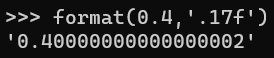
\includegraphics[scale=1]{recourses/repre04.png}
			\caption{Representación de 0.4 como float.\label{fig:code}}
		\end{center}
	\end{figure}
	
	\begin{figure}
		\begin{center}
			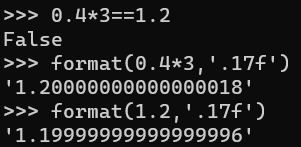
\includegraphics[scale=1]{recourses/comp04mult3.png}
			\caption{Comparación de números flotantes.\label{fig:code}}
		\end{center}
	\end{figure}
	
	Otro problema que debemos de tener en cuenta a la hora de trabajar con estas aproximaciones es la comparación de los números obtenidos, por ejemplo ilustremos la comparación mostrada en la Figura 6 donde podemos apreciar que en el sistema de coma flotante $0.4\cdot 3$ es ligeramente superior a 1.2. Por este motivo a la hora de trabajar con los números flotantes en el diseño de nuestros algoritmos siempre debemos tener en cuenta este error y evitar hacer comparaciones del tipo $a==b$, donde $a$ y $b$ son números flotantes.


%-----------------------------------------------------------------------------------
\subsection{Análisis de la Comparación}\label{sub:comp}
%-----------------------------------------------------------------------------------

	En esta sección analizaremos los resultados de los cálculos obtenidos al probar las distintas aritméticas con las funciones implementadas en \textbf{ArihmeticMath}, en cuanto a precisión numérica y tiempo de ejecución, dichos resultados se muestran en la sección \textbf{Tablas y Valores Obtenidos}.
	
%-----------------------------------------------------------------------------------
\subsubsection{Principales Funciones Matemáticas}\label{sub:math_func}
%-----------------------------------------------------------------------------------

	
	En la Figura 8 podemos observar las aproximaciones para sen($\pi$), por nuestros conocimientos matemáticos podemos percatarnos que el resultado es 0, sin embargo, observamos que las 3 aproximaciones arrojan valores ligeramente mayores a 0, con más exactitud para \textbf{FractionNum} y una mayor velocidad para \textbf{DecimalNum}.

	En la Figura 9 se comparan las aproximaciones para los números $\pi$ y $e$, respectivamente, con una mayor cantidad de cifras significativas para nuestra aritmética, aunque también con el tiempo más elevado, mientras \textbf{DecimalNum} sigue contando con el menor tiempo. 
	
	Pasamos a la Figura 10 donde comparamos el cálculo de ln($e$), podemos percatarnos de que \textbf{FractionNum} es la única que nos proporciona el resultado preciso, mientras nuestra aritmética cuenta con más exactitud que \textbf{DecimalNum}.
	
	Ahora procederemos a comparar potencias con índices decimales y raíces n-ésimas una tarea que puede ser computacionalmente más compleja, ya que como vimos annteriormente lleva el cálculo de potencias que pueden ser potencialmente más costosas que los factoriales utilizados en las series trigonométricas.
	
	En la Figura 12 se muestras el cálculo de $\sqrt{2}$, donde se aprecia una mayor exactitud en cuanto a decimales para nuestra aritmética pero para \textbf{FractionNum} ha sido imposible realizar el computo dentro de los límites de tiempo concebidos.
	
	En la Figura 13 se muestran los valores obtenidos para $\pi^{0.5}$, con mejor exactitud y velocidad para \textbf{DecimalNum}, al igual que en el análisis anterior ha sido imposible realizar los cálculos para \textbf{FractionNum}.
	
%-----------------------------------------------------------------------------------
\subsubsection{Comparando números}\label{sub:number_comp}
%-----------------------------------------------------------------------------------

	En esta sección analizaremos algunos de los ejemplos planteados en la sección donde describimos las limitaciones y los problemas de la coma flotante.
	
	\begin{figure}[h!]%
		\begin{center}
			\begin{tabular}{|c|c|c|} \hline
			 			 & $0.4\cdot 3==1.2$ 	    & $\sqrt{2}^3==2^{1.5}$ 	\\ \hline
			BigNum       &  True  & True     \\ \hline
			FractionNum  &  False &   -   \\ \hline
			DecimalNum   &  False & True   \\ \hline
						& $1.5\cdot 2==0.1+0.2$ 	    & $6/10==0.6$	\\ \hline
			BigNum       &  True  & True     \\ \hline
			FractionNum  &  False & False  \\ \hline
			DecimalNum   &  False & False  \\ \hline

\end{tabular}
		\caption{Comparando números. \label{fig:ex}}
		\end{center}
	\end{figure}
	
	En la Figura 7 podemos observar algunos de los ejemplos planteados en secciones anteriores, donde se demuestra la exactitud de nuestra biblioteca antes estos escenarios y los problemas del sistema de coma flotante.
  
	
	
\onecolumn
%-----------------------------------------------------------------------------------
\subsection{Tablas y Valores Obtenidos}\label{sub:table}
%-----------------------------------------------------------------------------------
	
	\begin{figure}[h!]%
		\begin{center}
			\begin{tabular}{|c|c|l|l|} \hline
			
			&Calculo de:
			& Valor 	    
			& Tiempo	
			\\ \hline
					
	BigNum	& sen($\pi$)	
		    	& 0.00000000000000023846264338327950288419718393539484659  
		    & 0.0276847    
		    \\ \hline
		    
FractionNum 	& sen($\pi$)	
			& 1.2246467991473532e-16                                   			& 0.00103831   
			\\ \hline
			
DecimalNum  	& sen($\pi$)
			& 1.224646799150525701746457189E-16                        			& 6.19888e-05  
			\\ \hline

 	BigNum  	& sen(1)	  															   	& 0.841470984807896506652502321630298999622563060798371067
 			& 0.0127552    
 			\\ \hline
 			
FractionNum 	& sen(1)
			& 0.8414709848078965                                        			& 0.000446081  
			\\ \hline
			
DecimalNum  	& sen(1)
			& 0.8414709848078965066525023216                            			& 5.31673e-05  
			\\ \hline
			
	BigNum  & cos(10)
			&-0.839071529076449284094014962603313164795669011492621151  			& 0.0178885    
			\\ \hline
			
FractionNum 	& cos(10) 
			& -0.8390715290764493                                        			& 0.000496149  
			\\ \hline
			
DecimalNum  	& cos(10) 
			& -0.8390715290764492840940147683                            			& 5.45979e-05  
			\\ \hline
			
	BigNum  	& cos($\pi\over 2$)  										
			& 0.000000000000000019231321691639751442098584699687551724  
			& 0.0247827   
			\\ \hline
			
FractionNum 	& cos($\pi\over 2$)
			& 6.123233995736766e-17                                     			& 0.00112844  
			\\ \hline
			
DecimalNum  	& cos($\pi\over 2$)
			& 6.123233995815319195807292141E-17                         			& 6.1512e-05  
			\\ \hline
			
\end{tabular}
		\caption{Cálculo de funciones trigonométricas. \label{fig:ex}}
		\end{center}
	\end{figure}
	
	
	\begin{figure}[h!]%
		\begin{center}
			\begin{tabular}{|c|c|l|l|} \hline
			
			&Calculo de:
			& Valor 	    
			& Tiempo	
			\\ \hline
			
	BigNum  	& $\pi$
			& 3.141592653589793238462643383279502884197169399375105588  			& 0.174473     
			\\ \hline
			
FractionNum 	& $\pi$
			& 3.141592653589793                                         			& 0.00294471   
			\\ \hline
			
DecimalNum  	& $\pi$ 
			& 3.141592653589793238462643381                             			& 0.000238657  
			\\ \hline
			
	BigNum  	& $e$
			& 2.718281828459045235360287471352662497757247093698703317  			& 0.0109069    
			\\ \hline
			
FractionNum 	& $e$
			& 2.718281828459045                                         			& 0.000371218  
			\\ \hline
			
DecimalNum  	& $e$
			& 2.718281828459045235360287474                             			& 4.31538e-05  
			\\ \hline

\end{tabular}
		\caption{Cálculo de $\pi$ y $e$. \label{fig:ex}}
		\end{center}
	\end{figure}
	
	
	\begin{figure}[h!]%
		\begin{center}
			\begin{tabular}{|c|c|l|l|} \hline
			
			&Calculo de:
			& Valor 	    
			& Tiempo	
			\\ \hline
			
	BigNum  	& ln(34)  
			& 3.524193849218783867017024061131077780596772055958075561  			& 0.0921957    
			\\ \hline
			
FractionNum 	& ln(34)
			& 3.5241938492187836                                        			& 0.00212646   
			\\ \hline
			
DecimalNum  	& ln(34)
			& 3.524193849218783867017024054                             			& 0.000117302  
			\\ \hline
			
	BigNum  	& ln($e$)
			& 0.999999999999999913415788971088737539870366147960492922  			& 0.0782981    
			\\ \hline
			
FractionNum 	& ln($e$)
			& 1.0                                                       			& 0.0125442    
			\\ \hline
			
DecimalNum  	& ln($e$)
			& 0.9999999999999999468176229340                            			& 0.000138283  
			\\ \hline


\end{tabular}
		\caption{Cálculo de ln($x$). \label{fig:ex}}
		\end{center}
	\end{figure}
	
	
	\begin{figure}[h!]%
		\begin{center}
			\begin{tabular}{|c|c|l|l|} \hline
			
			&Calculo de:
			& Valor 	    
			& Tiempo	
			\\ \hline
			
	BigNum  	& atan(20)
			& 3.091634257867850477052637096244658002705892318951598412  			& 0.293755   
			\\ \hline
			
FractionNum 	& atan(20)
			& 3.0916342578678506                                        			& 0.155865   
			\\ \hline
			
DecimalNum  	& atan(20)
			& 3.091634257867850477052637094                             			& 0.0010519  
			\\ \hline
			
	BigNum  	& asin(1)
			& 1.514354028437096828855179419136122881185661180257748239  			& 0.130738     
			\\ \hline
			
FractionNum 	& asin(1)
			& 1.5143540284370969                                        			& 0.00287724   
			\\ \hline
			
DecimalNum 	& asin(1)
			& 1.514354028437096828855179423                             			& 0.000198841  
			\\ \hline


\end{tabular}
		\caption{Cálculo de funciones trigonométricas inversas. \label{fig:ex}}
		\end{center}
	\end{figure}	

\newpage
	
	\begin{figure}[h!]%
		\begin{center}
			\begin{tabular}{|c|c|l|l|} \hline
			
			& Calculo de:
			& Valor 	    
			& Tiempo	
			\\ \hline
		
	BigNum 	& $\sqrt[12]{45}$
			& 1.373307239498335812855818924624660567276647132735873217  
			& 0.305376     
			\\ \hline
			
FractionNum 	& $\sqrt[12]{45}$
			&  -  
			&  -     
			\\ \hline
			
DecimalNum  	& $\sqrt[12]{45}$  
			& 1.373307239498335812855818925                             
			& 0.000169277  
			\\ \hline
			
	BigNum  	& $\sqrt{2}$
			& 1.414213562373095048801688724209698078569671875376948073  
			& 0.0293512   
			\\ \hline
			
FractionNum 	& $\sqrt{2}$  
			& -   
			& -
			\\ \hline
			
DecimalNum 	& $\sqrt{2}$
			& 1.414213562373095048801688724                             
			& 0.00041008  
			\\ \hline

			
\end{tabular}
		\caption{Cálculo de raíces n-ésimas. \label{fig:ex}}
		\end{center}
	\end{figure}	
	
	
	\begin{figure}[h!]%
		\begin{center}
			\begin{tabular}{|c|c|l|l|} \hline
				
			& Calculo de:
			& Valor 	    
			& Tiempo	
			\\ \hline
		
	BigNum 	& $\pi^{0.5}$
			& 1.772453850905515960029097752286351896216738465831096675  
			& 0.0269032    
			\\ \hline
			
FractionNum 	& $\pi^{0.5}$  
			& -     
			& -
			\\ \hline
			
DecimalNum 	& $\pi^{0.5}$
			& 1.772453850905515992751519103                             
			& 8.70228e-05  
			\\ \hline
			
	BigNum  	& $3^{4.5}$ 	
			& 140.296115413079060775723153661975661722367225558640830762  
			& 0.0319946    
			\\ \hline
			
FractionNum	& $3^{4.5}$ 
			& -  				
			& -    
			\\ \hline
			
DecimalNum  	& $3^{4.5}$
			& 140.2961154130790607757231540                               				& 9.46522e-05  
			\\ \hline


\end{tabular}
		\caption{Cálculo de potencias con índices no enteros. \label{fig:ex}}
		\end{center}
	\end{figure}
	
	
	
\twocolumn

%-----------------------------------------------------------------------------------
\subsection{Sacando lo máximo de nuestra aritmética}\label{sub:big}
%-----------------------------------------------------------------------------------
	
	En esta sección mostraremos los reultados obtenidos en el desempeño de nuestra aritmética para tareas computacionalmente complejas, como la aproximación de $\pi$ y $e$ con varias cifras decimales y el cálculo de números grandes como los factoriales.
	
	\begin{figure}[h!]%
		\begin{center}
			\begin{tabular}{|c|c|c|} \hline
			 	Cifras Correctas & Tiempo 	\\ \hline
			    100              &  1.357109 \\ \hline  
			    200              &  5.720520  \\ \hline
				500              &  30.96164  \\ \hline

\end{tabular}
		\caption{Aproximación de los decimales de $\pi$. \label{fig:ex}}
		\end{center}
	\end{figure}
	
	\begin{figure}[h!]%
		\begin{center}
			\begin{tabular}{|c|c|c|} \hline
			 	Cifras Correctas & Tiempo 	\\ \hline
			    100              &  0.047280 \\ \hline  
			    200              &  0.127560  \\ \hline
				500              &  0.887334  \\ \hline

\end{tabular}
		\caption{Aproximación de los decimales de $e$. \label{fig:ex}}
		\end{center}
	\end{figure}
	
	\begin{figure}[h!]%
		\begin{center}
			\begin{tabular}{|c|c|c|} \hline
			 	Factorial & Tiempo 	\\ \hline
			    100              &  0.027119 \\ \hline  
			    1000             &  3.804981  \\ \hline
				10000            &  457.1413  \\ \hline
		
\end{tabular}
		\caption{Cálculo de factoriales. \label{fig:ex}}
		\end{center}
	\end{figure}
	
	Además mostremos la utilización de nuestra aritmética en algoritmos iterativos para la resolución de equaciones lineales, para ello resolvamos el siguiente sistema de equaciones por el \textbf{Metódo de Jacobi} y el \textbf{Metódo de Gauss-Seidel}.
	
	\begin{equation}	
		\left(	
		\begin{matrix}
			9  &  3  &  4\\
            	-3 &  7  & -3\\
            	2  &  2  &-10 
		\end{matrix}
		\quad\Bigg|\quad
		\begin{matrix}
			1\\
			1\\
			1\\
		\end{matrix}
		\right)
	\end{equation}
	
	Obteniendo como resultado el siguiente vector para el \textbf{Metódo de Jacobi}:
	$$	
		\left(	
		\begin{matrix}
			0.08246073298429319371727748691099476439790\\ 								0.15575916230366492146596858638743455497382\\ 								-0.05235602094240837696335078534031413612565\\
		\end{matrix}
		\right)
	$$ con un tiempo de ejecución de 1.8970699310302734 segundos.
	
	Obteniendo como resultado el siguiente vector para el \textbf{Metódo de Gauss-Seidel}:
	$$	
		\left(	
		\begin{matrix}
			0.08246073298429319371727748691099476439790\\ 								0.15575916230366492146596858638743455497382\\ 								-0.05235602094240837696335078534031413612565\\
		\end{matrix}
		\right)
	$$ con un tiempo de ejecución de 1.7851269245147705 segundos.
	
%-----------------------------------------------------------------------------------
\subsection{Finalizando Comparaciones}\label{sub:big}
%-----------------------------------------------------------------------------------
	En las diferentes secciones abordadas de este tema, nos percatamos de que los resultados favorecen en cuanto a precisión favorecen a \textbf{BigNum} aunque por un estrecho margen. Sin embargo en el caso de los cálculos de expresiones decimales no finitas todas las aritméticas ofrecen comportamientos similares, con algunas ventajas para \textbf{FractionNum} como vimos en un ejemplo aunque vale la pena señalar que se realizó una división en todos los casos del numerador entre el divisor para poder comparar los resultados con las demás artiméticas, por lo cual no se explota todo el potencial de esta.
	
	En cuanto a los tiempos de ejecución la aritmética más eficiente es \textbf{DecimalNum}, \textbf{FractionNum} en este sentido se vio incapacitada de realizar algunos cálculos, mientras que nuestra aritmética si bien fue la menos eficiente en la mayoría de los casos, no se obtuvieron tiempos dentro de lo razonable para la ejecución de un algoritmo.
	
	En la última sección analizada podemos observar la eficiencia de nuestra aritmética ante escenarios complejos desde el punto de vista computacional.


	

%-----------------------------------------------------------------------------------
	\subsection{Referencias}
%-----------------------------------------------------------------------------------
  	Las referencias deben estar agrupadas en una sección al final del artículo,
  	y las citas numeradas correctamente, por ejemplo \cite{knuth} o \cite{goedel}.
  	Incluya toda la información importante de cada referencia, incluídos autor,
  	título, y notas de la edición. En caso de citar sitios web, además
  	de la URL, incluya la fecha en que fue consultado, como en \cite{wiki}. Numere 
  	las referencias según el orden en que se les cita.

%===================================================================================



%===================================================================================
% Conclusiones
%-----------------------------------------------------------------------------------
\section{Conclusiones}\label{sec:conc}

  En nuestro análisis del desempeño de la aritmética propuesta en este trabajo se vio reflejada la exactitud que esta posee a la hora de trabajar con datos de números en base 10. No obstante simepre tuvimos la desventaja de que la aritmética de punto flotante analizada fuera más rápida y eficiente y en par de ejemplos superando la exactitud de la nuestra. Por otro lado, observamos el comportamiento de la aritmética de fracciones racionales, si bien incapacitada de todo su potencial a la hora de compararse con las anteriores por los problemas antes explicados, siendo más precisa que las 2 anteriores en algunos casos, aunque incapacitada para realizar algunas tareas también especificadas anteriormente.
  
  Cabe recalcar que la mayoría de estas comparaciones realizadas anteriormente en cuanto a la exactitud también se debe en gran medida a los métodos numéricos en los cuales se basa su cálculo, por lo que otro método numérico, fuera de los aquí abordados, pudiera ser más efectivo en uno u otro caso. 
  
  Por tanto, por todo lo anteriormente descrito podemos concluir que las aritméticas de punto flotante, si bien pueden tener su desventaja a la hora de la precisión y exactitud, actualmente es el método más efectivo para la realización de los cálculos computacionales.

%===================================================================================



%===================================================================================
% Recomendaciones
%-----------------------------------------------------------------------------------
\section{Recomendaciones}\label{sec:rec}

  En esta sección puede incluir recomendaciones sobre posibles formas de continuar
  la investigación u otros temas relacionados.

%===================================================================================



%===================================================================================
% Bibliografía
%-----------------------------------------------------------------------------------
\begin{thebibliography}{99}
%-----------------------------------------------------------------------------------
	\bibitem{wiki} Algorithm D. URL: \href{https://ridiculousfish.com/blog/posts/labor-of-division-episode-iv.html}
	  {https://ridiculousfish.com/blog/posts/labor-of-division-episode-iv.html}.
		Consultado en 19 de noviembre de 2022.
		
	\bibitem{wiki} Algoritmo para calcular la raíz n. URL: \href{https://es.frwiki.wiki/wiki/Algorithme_de_calcul_de_la_racine_n-i\%C3\%A8me}
	  {https://es.frwiki.wiki/wiki/Algorithme\_de\_calcul\_de\_la\_racine\_n-i\%C3\%A8me}.
		Consultado en 19 de noviembre de 2022.
	
	\bibitem{wiki} IEEE-174-1985. Wikipedia. URL: \href{https://en.wikipedia.org/wiki/IEEE_754-1985}
	  {https://en.wikipedia.org/wiki/IEEE\_754-1985}.
		Consultado en 19 de noviembre de 2022.
		
	\bibitem{wiki} Karatsuba algorithm. Wikipedia. URL: \href{https://en.wikipedia.org/wiki/Karatsuba_algorithm}
	  {https://en.wikipedia.org/wiki/Karatsuba\_algorithm}.
		Consultado en 19 de noviembre de 2022.	
		
	\bibitem{wiki} Taylor Series. Wikipedia. URL: \href{https://en.wikipedia.org/wiki/Taylor_series}
	  {https://en.wikipedia.org/wiki/Taylor\_series}.
		Consultado en 19 de noviembre de 2022.
		
	
	
	
	

%-----------------------------------------------------------------------------------
\end{thebibliography}

%-----------------------------------------------------------------------------------

\label{end}

\end{document}

%===================================================================================
